\subsection{Machine Learning Model Diagram}
\label{subsec:ml_diagram}
In this section, the process on how the machine learning model 
was developed is shown in Figure \ref{fig:ml_model}. 
Wherein, the process overview is based on the Fine-Tuned Support 
Vector Regression Model for Stock Predictions by 
\citeA{Dash2016}.
% Machine Learning Model Diagram
\begin{figure}[ht]
    \centering
    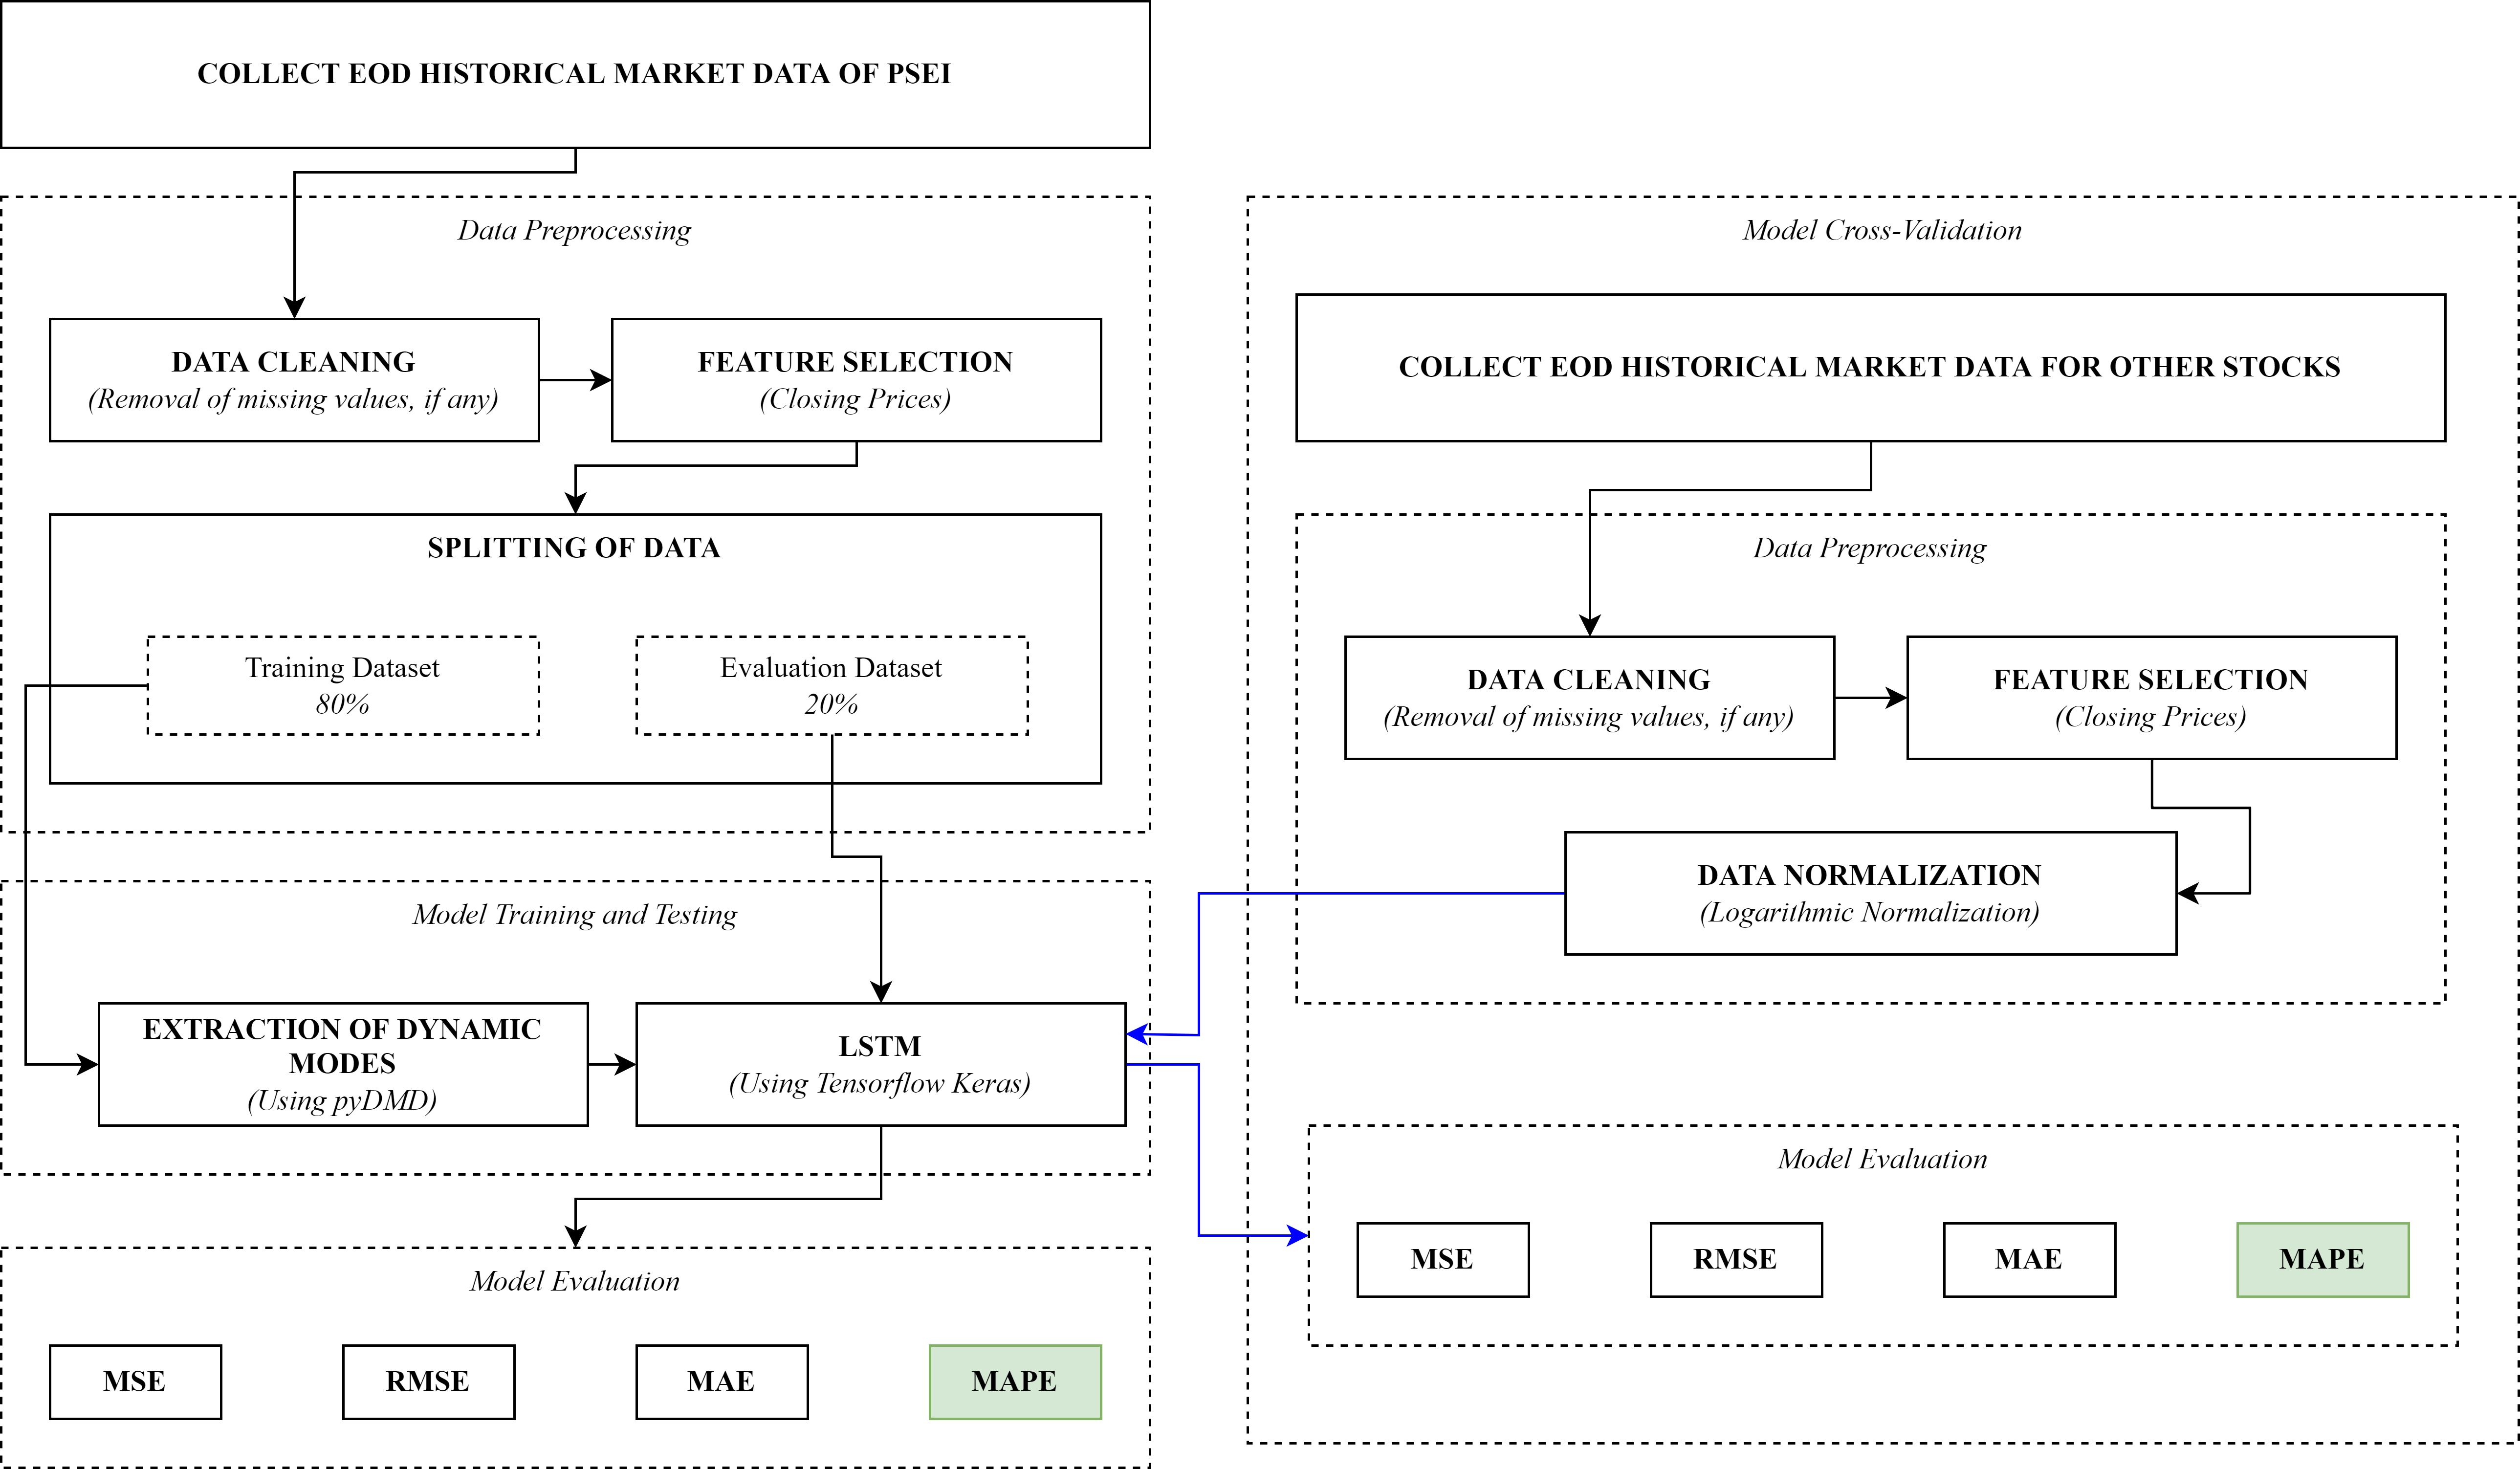
\includegraphics[width=1\textwidth]{./assets/Chapter_3/Machine Learning Model.png}
    \caption{Machine Learning Model for the alamSYS}
    \label{fig:ml_model}
\end{figure}
\FloatBarrier

\subsubsection{Data Collection}
\label{subsubsec:model_data_collection}
The market data used to develop the DMD-LSTM model was obtained through EODHD's 
end-of-day market data API. While PSEI market data was used for model 
training and testing, market data from other stocks was used for cross-validation 
of the DMD-LSTM model. The following are the specifics of the stocks gathered:
\begin{longtable}{|c|c|c|c|}
    \caption{Collected Market Data Details}
    \label{tab:market_data_details}\\
    \hline
    \textbf{Stock} & \textbf{Data Count} & \textbf{Start Date} & \textbf{End Date} \\ \hline
    \endfirsthead
    %
    \multicolumn{4}{c}%
    {{\bfseries Table \thetable\ continued from previous page}} \\
    \hline
    \textbf{Stock} & \textbf{Data Count} & \textbf{Start Date} & \textbf{End Date} \\ \hline
    \endhead
    %
    \textbf{AC}    & 6809                & June 27, 1994       & February 10, 2023 \\ \hline
    \textbf{ALI}   & 6789                & June 27. 1994       & February 10, 2023 \\ \hline
    \textbf{AP}    & 3795                & July 16, 2007       & February 10, 2023 \\ \hline
    \textbf{BDO}   & 5041                & May 22, 2002        & February 10, 2023 \\ \hline
    \textbf{BLOOM} & 3033                & October 30, 2000    & February 10, 2023 \\ \hline
    \textbf{FGEN}  & 4142                & February 02, 2006   & February 10, 2023 \\ \hline
    \textbf{GLO}   & 6707                & January 03, 1995    & February 10, 2023 \\ \hline
    \textbf{ICT}   & 6805                & January 03, 1995    & February 10, 2023 \\ \hline
    \textbf{JGS}   & 6525                & June 27, 1994       & February 10, 2023 \\ \hline
    \textbf{LTG}   & 3774                & February 06, 1995   & February 10, 2023 \\ \hline
    \textbf{MEG}   & 6751                & January 03, 1995    & February 10, 2023 \\ \hline
    \textbf{MER}   & 6799                & June 27, 1994       & February 10, 2023 \\ \hline
    \textbf{MPI}   & 3888                & December 18, 2006   & February 10, 2023 \\ \hline
    \textbf{PGOLD} & 2762                & October 06, 2011    & February 10, 2023 \\ \hline
    \rowcolor[HTML]{9AFF99} 
    \textbf{PSEI}  & 5675                & January 03, 2000    & February 10, 2023 \\ \hline
    \textbf{RLC}   & 5879                & June 27, 1994       & February 10, 2023 \\ \hline
    \textbf{RRHI}  & 2253                & November 11, 2013   & February 10, 2023 \\ \hline
    \textbf{SMC}   & 6799                & June 27. 1994       & February 10, 2023 \\ \hline
    \textbf{TEL}   & 6814                & June 27, 1994       & February 10, 2023 \\ \hline
    \textbf{URC}   & 6135                & June 03, 1995       & February 10, 2023 \\ \hline
\end{longtable}

\subsubsection{Data Preprocessing}
\label{subsubsec:model_data_processing}
Data preprocessing is composed of three main processes which are as follows:
\begin{itemize}
    \item[(a)] Data Cleaning - This was done to clean any missing values from the data.
    \item[(b)] Feature Selection - Closing prices was selected as the main feature of the model.
    \item[(c)] Splitting of Data - Data was split 80:20 for testing and training data, respectively.
\end{itemize}

\subsubsection{Model Training and Testing}
\label{subsubsec:model_training_testing}
xxx

\subsubsection{Model Cross-Validation}
\label{subsubsec:model_cross_validation}
xxx

\subsubsection{Model Evaluation}
\label{subsubsec:model_evaluation}
xxx

\subsubsection{Model Deployment}
\label{subsubsec:model_deployment}
xxx